%============================
% SECTION 8: SUMMARY
%============================
\section{Summary}

\begin{frame}
\frametitle{Complete Pipeline}

\begin{center}
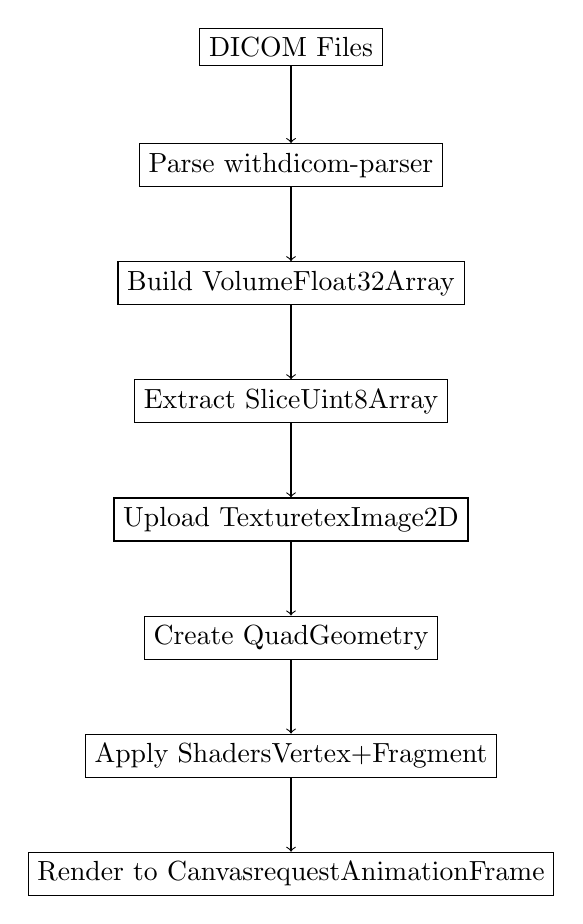
\begin{tikzpicture}[node distance=1.5cm, auto, scale=0.9]
  \node[draw, rectangle] (dicom) {DICOM Files};
  \node[draw, rectangle, below of=dicom] (parse) {Parse with\\dicom-parser};
  \node[draw, rectangle, below of=parse] (volume) {Build Volume\\Float32Array};
  \node[draw, rectangle, below of=volume] (slice) {Extract Slice\\Uint8Array};
  \node[draw, rectangle, below of=slice] (texture) {Upload Texture\\texImage2D};
  \node[draw, rectangle, below of=texture] (quad) {Create Quad\\Geometry};
  \node[draw, rectangle, below of=quad] (shader) {Apply Shaders\\Vertex+Fragment};
  \node[draw, rectangle, below of=shader] (render) {Render to Canvas\\requestAnimationFrame};
  
  \draw[->] (dicom) -- (parse);
  \draw[->] (parse) -- (volume);
  \draw[->] (volume) -- (slice);
  \draw[->] (slice) -- (texture);
  \draw[->] (texture) -- (quad);
  \draw[->] (quad) -- (shader);
  \draw[->] (shader) -- (render);
\end{tikzpicture}
\end{center}
\end{frame}

\begin{frame}
\frametitle{Key Technologies}

\begin{columns}
\column{0.5\textwidth}
\textbf{Frontend}
\begin{itemize}
  \item React + TypeScript
  \item Interactive UI controls
  \item Real-time slice selection
\end{itemize}

\textbf{Medical Data}
\begin{itemize}
  \item DICOM file format
  \item Multi-file volume assembly
  \item Hounsfield units
\end{itemize}

\column{0.5\textwidth}
\textbf{Graphics}
\begin{itemize}
  \item WebGL 1.0
  \item GPU texture storage
  \item Shader programming
\end{itemize}

\textbf{3D Math}
\begin{itemize}
  \item Matrix transformations
  \item Camera controls
  \item Orthogonal projections
\end{itemize}
\end{columns}
\end{frame}

\begin{frame}
\frametitle{Performance Characteristics}

\textbf{Memory Usage:}
\begin{itemize}
  \item Volume storage: $W \times H \times D \times 4$ bytes (Float32)
  \item Example: $512 \times 512 \times 200$ = 209 MB
  \item Texture: $W \times H$ (slice) = 262 KB
\end{itemize}

\vspace{0.3cm}

\textbf{Computational Complexity:}
\begin{itemize}
  \item Parse single DICOM: $O(n)$ bytes
  \item Build volume: $O(W \times H \times D)$
  \item Extract slice: $O(W \times H)$ or $O(W \times D)$
  \item Render frame: Real-time (GPU-accelerated)
\end{itemize}

\vspace{0.3cm}

\textbf{Optimizations:}
\begin{itemize}
  \item Lazy slice extraction (on-demand)
  \item GPU texture filtering (linear interpolation)
  \item requestAnimationFrame for efficient rendering
\end{itemize}
\end{frame}

\begin{frame}
\frametitle{Advantages of This Approach}

\begin{itemize}
  \item \textbf{GPU Acceleration}: Fast rendering of slices
  \item \textbf{Interactive}: Real-time slice navigation
  \item \textbf{Web-based}: No installation required
  \item \textbf{Standard Format}: Works with DICOM from any modality
  \item \textbf{Extensible}: Easy to add volume rendering, MPR, etc.
  \item \textbf{Cross-platform}: Works on desktop and mobile
\end{itemize}
\end{frame}

\begin{frame}
\frametitle{Future Enhancements}

\begin{itemize}
  \item \textbf{Volume Rendering}: Raycasting for 3D visualization
  \item \textbf{Windowing}: Intensity range control (Hounsfield units)
  \item \textbf{Measurements}: Distance, angle, area tools
  \item \textbf{Annotations}: Drawing tools for clinical notes
  \item \textbf{WebGL2}: Advanced shaders, compute
  \item \textbf{Multi-File}: Temporal sequences (4D)
  \item \textbf{Export}: Save processed images/videos
\end{itemize}
\end{frame}

\begin{frame}
\frametitle{Questions?}

\begin{center}
\Large
Thank you for your attention!

\vspace{1cm}

Code available at:\\
\texttt{github.com/rathoddinesh14/graphicus-harena}

\vspace{1cm}

Key Resources:
\begin{itemize}
  \item Khronos WebGL Specification
  \item DICOM Standard Documentation
  \item Medical Image Processing: Gonzalez \& Woods
\end{itemize}
\end{center}
\end{frame}